\documentclass{report}
\usepackage[dutch]{babel}
\usepackage{amsmath}
\usepackage{amssymb}
\usepackage{fixltx2e} % overbodig?
\usepackage{caption}
\usepackage{subcaption}
\usepackage[toc,page]{appendix}
\usepackage{verbatim}
\usepackage{url}
\usepackage{ragged2e}
\usepackage[numbered]{mcode}
\usepackage{wallpaper} %voor voorpagina

% Voor plaatje(s)
\usepackage{graphicx}
\usepackage{tikz}
\usepackage{wrapfig}
\usepackage{datetime}
\usepackage[nomessages]{fp}
\usepackage{float}

\title{Rivier oversteken}
\date{\today}
\author{Casper Barendrecht\\ Bram van den Heuvel \\ Arnoud van der Leer \\ Reena Sitaram}

\begin{document}
	%\maketitle	
	
	\LRCornerWallPaper{2.3}{Segregation.jpg}
\LRCornerWallPaper{1}{LeidenLogo.png}
\LLCornerWallPaper{1}{tudelft.pdf}


% In de onderstaande renews kunnen naar voorkeur de logos worden verplaatst op een niet hele nette manier
\begin{comment}
%hieronder kan in hspace\vspace de locatie van het leiden logo worden verplaatst. Een lelijke manier maar werkt voor nu :) 
\renewcommand{\ThisLRCornerWallPaper}[2]{%
  \AddToShipoutPicture*{%
    \AtPageLowerLeft{%
      \parbox[b]{\paperwidth}{%       
        \hfill \includegraphics[width=#1\paperwidth,height=#1\paperheight,%
        keepaspectratio]{#2}%
	\hspace{1cm}\vspace{0.5cm}
      }
    }
  }
}

%Analoog vor het TU Delft Logo
\renewcommand{\ThisLLCornerWallPaper}[2]{%
\AddToShipoutPicture*{%
  \AtPageLowerLeft{%
  	\parbox[b]{\paperwidth}{%
		\hspace{0.8cm}    
   	 	\includegraphics[width=#1\paperwidth,height=#1\paperheight,%
    	  keepaspectratio]{#2}%
		\vspace{0.5cm}    
	}
   }
  }
}
\end{comment}

\begin{titlepage}

	\LRCornerWallPaper{2.3}{boot1.jpg}

	\centering
	{\scshape\Large Technische Universiteit Delft\par}
	\vspace{1cm}
	{\scshape\Large Modelleren 1B\par}
	\vspace{1.5cm}
	{\Huge\bfseries Rivier Oversteken\par}
	\vspace{2cm}
	{\Large
	C. Barendrecht\\ 
	B. van den Heuvel\\
	A. van der Leer\\
	R.Sitaram\par}
	\vfill
	Onder begeleiding van:\par
	Dr.~B. Meulenbroek

	\vfill
\end{titlepage}
\ClearWallPaper	
	
	\chapter*{Lijst met gebruikte symbolen}
\begin{tabular}{ l l }
	\(a\) & De constante die een gewicht geeft aan tijd en energie in de kostenfunctie\\
	\(a\) & Een stromingsconstante die de sterkte van een stromingsprofiel bepaalt\\
	\(A\) & Het oppervlakte van een dwarsdoorsnede van een rivier\\
	\(A_{gem}\) & Het gemiddelde oppervlakte van de dwarsdoorsnedes van een rivier\\
	\(c\) & De wrijvingsconstante\\
	\(C(t)\) & De kostenfunctie\\
	\(\mathcal{C}\) & Het pad dat word afgelegd door de boot\\
	\(E(t)\) & De totale hoeveelheid energie op tijdstip \(t\)\\
	\(F\) & De kracht die verricht word door de boot\\
	\(F_w\) & De wrijvingskracht die verricht word op de boot\\
	\(\widetilde{F}\) & De som van de krachten die op de boot werken\\
	\(m\) & De massa van de boot\\
	\(Q\) & De waterverplaatsing van een rivier \\
	\(Q_{gem}\) & De gemiddelde waterverplaatsing van een rivier\\
	\(s\) & De stromingsconstante bij een constante stroming\\
	\(S(x_1)\) & De stroming op lijn \(x_1\)\\
	\(T\) & Tijd van aankomst bij de bestemming\\
	\(u(t)\) &	De stuurrichting als functie van de tijd\\
	\(v(t)\) & De snelheid van de boot\\
	\(\overrightarrow{v}\) & De snelheidsvector van een rivier\\
	\(v_{gem}\) & De gemiddelde snelheid van een rivier\\
	\(x_1\) & De horizontale as\\
	\(x_2\) & De verticale as\\
	\(x_1(t)\) & De horizontale positie van de boot op tijdstip \(t\)\\
	\(x_2(t)\) & De verticale positie van de boot op tijdstip \(t\)\\
	\(\mu\) & De functie die de verhouding tussen \(\lambda_1\) en \(\lambda_2\) aangeeft. (Zie pagina \pageref{mu})
\end{tabular}
	

	\chapter*{Voorwoord}
Dit rapport is geschreven door Bram van den Heuvel, Casper Barendrecht, Arnoud van der Leer en Reena Sitaram, eerstejaars studenten Wiskunde aan de TU Delft en Leiden Universiteit. Het doet verslag van een onderzoeksproject dat wij uitvoerden voor het vak Modelleren-1B. Bij dit onderzoek zijn wij begeleid door Bernard Meulenbroek.

Wij kozen ervoor een model te maken dat een boot beschrijft die een rivier oversteekt. Het is ons goed gelukt de basisversie van het probleem uit te werken. Door gebrek aan tijd is het niet gelukt de uitbreiding volledig af te ronden. 

Wij willen onze begeleider van harte danken voor zijn betrokkenheid en goede tips; wanneer wij niet wisten hoe we verder moesten wist hij ons steeds in de goede richting te sturen.

{\raggedleft{\emph{\small{Casper Barendrecht, Bram van den Heuvel, Arnoud van der Leer en Reena Sitaram}}}\\
\raggedleft{\emph{Delft, Mei 2016}}\\}


	\setcounter{tocdepth}{1}
	\tableofcontents

	\chapter{Inleiding}
Transport over water is essentieel voor de wereldeconomie; meer dan 90\% van alle handel wordt gefaciliteerd door maritiem transport \cite{wereldwijdeHandel}. Dat is geen toeval: transport over water is de efficientste vorm van transport over lange afstanden \cite{efficientstTransport}. Het kiezen van een goede route is een integraal onderdeel van deze efficientie.

Wij introduceren een model waarmee we op zoek gaan naar een route tussen twee locaties. Eerst zoeken we naar de snelste route, daarna breiden we ons model uit en zoeken we naar de goedkoopste route.

Het eerste model beschrijft een boot welke met constante vaarsnelheid een stuk water moet oversteken. 
De stroming van dit water is gegeven door een continu stromingsprofiel. 
Er kan alleen gevarieerd worden in de stuurrichting en we zijn dus op zoek naar een functie die een stuurhoek beschrijft z\'o dat een kortste route afgelegd wordt. Eerst onderzoeken we ons model met een constant stromingsprofiel analytisch en vervolgens gaan we op zoek naar de snelste route voor een algemene stromingsfunctie. Hiervoor gebruiken we een combinatie van analytische en numerieke methoden.

Het tweede model is een uitbreiding op de eerste. Waar het eerste model een constante vaarsnelheid aannam kiezen we er nu voor de snelheid te laten varieren afhankelijk van een stuwkracht. We zoeken nu naar een route die niet alleen snel is maar ook weinig energie gebruikt. Afhankelijk van een parameter kan de verhouding tussen de kosten van energie en de kosten van tijd worden gekozen. Wederom gebruiken we analytische en numerieke methoden om de goedkoopste route te vinden. Het onderzoek naar dit tweede model wordt deels voltooid.

	
	\chapter{Situatieschets}\label{sec:situatieschets}

\begin{wrapfigure}{r}{4.5cm}
	\usetikzlibrary{calc}
\begin{tikzpicture}[scale = 3.5, transform shape]
	% Variables
	\newcommand{\boatAngle}{25}
	\newcommand{\vectorLength}{.25}
	\newcommand{\textSize}{.15}

	% River banks
	\draw (0, 1) -- (0, -1);
	\draw (1, 1) -- (1, -1);
	
	% Coordinate system
	\draw[->, thick] (0, 0) -- (1, 0);
	\draw[->, thick] (0, 0) -- (0, 1);
	
	% Coordinate system labels. The scope structures are used to make the text smaller.
	\begin{scope}[shift={(1, 0)}]
		\begin{scope}[scale=\textSize * 1.5, transform shape]
			\node[anchor=north east, font=\fontsize{10}{3}] at (0, 0) {$ x_1 $};
		\end{scope}
	\end{scope}
	\begin{scope}[shift={(0, 1)}]
		\begin{scope}[scale=\textSize * 1.5, transform shape]
			\node[anchor=north east, font=\fontsize{10}{3}] at (0, 0) {$ x_2 $};
		\end{scope}
	\end{scope}
	
	% Vector field
	\newcommand{\xVectors}{5} % Number of vectors in the x_1 direction
	\newcommand{\yVectors}{3} % Number of vectors in the x_2 direction
	\FPeval\xVectorsr{\xVectors - .5} % Each x_1 vector lies exactly between two integers
	\FPeval\yVectorsStart{1 - \yVectors} % The first y vector has to be one higher in order to have the lowest vectors inside the picture. 
	\foreach \x in {.5, ..., \xVectorsr} {
		\foreach \y in {\yVectorsStart, ..., \yVectors} {
			\FPeval\vectorLength{sin(\x/\xVectors * pi) / \yVectors / 2} % The length of the vector at \x, \y, calculated with a sine function.
			\draw[->, draw=gray!75!white, very thin] (\x/\xVectors, \y/\yVectors) -- (\x/\xVectors, \y/\yVectors - \vectorLength);
		}
	}
	
	% s(x_1) label
	\begin{scope}[shift={(.5, .9)}]
		\begin{scope}[scale=\textSize, transform shape]
			\node[anchor=west, font=\fontsize{10}{3}] at (0, 0) {$ s(x_1) $};
		\end{scope}
	\end{scope}
	
	% Boat center coordinate
	\coordinate (c) at (.3, .1);
	
	% Dashed boat path
	\draw[draw=gray, dashed] (0, 0) .. controls (.15, .02) .. (c) .. controls (.65, .26) .. (1, 0);
	
	% A scope to rotate and shift the boat
	\begin{scope}[rotate = \boatAngle, shift = {(c)}]
		% Boat outline
		\draw (.2, 0) .. controls (.15, -.05) .. (.1, -.05) -- (-.1, -.05) -- (-.1, .05) -- (.1, .05) .. controls (.15, .05) .. (.2, 0);
		
		% Boat direction vector
		\draw[->] (0, 0) -- (\vectorLength, 0);
		
		% v label
		\begin{scope}[shift={(\vectorLength/2, 0)}]
			\begin{scope}[scale=\textSize, transform shape]
				\node[anchor=south, font=\fontsize{10}{3}] at (0, 0) {$ v $};
			\end{scope}
		\end{scope}
		
		% Base line (for boat direction)
		\draw (0, 0) -- (-\boatAngle:\vectorLength);
		
		% Boat direction arc
		\draw (0:\vectorLength / 3 * 2) arc (0:-\boatAngle:\vectorLength / 3 * 2);
		
		% Boat center dot
		\draw[fill] (0, 0) circle (.01);
	\end{scope}
	
	% u label
	\begin{scope}[shift={($ (c) + (\boatAngle/2:\vectorLength/3*2) $)}]
		\begin{scope}[scale=\textSize, transform shape, rotate=\boatAngle/2]
			\node[anchor=west, font=\fontsize{10}{3}] at (0, 0) {$ u $};
		\end{scope}
	\end{scope}
	
\end{tikzpicture}
	\caption{De situatie}\label{fig:rivierplaatje}
\end{wrapfigure}

In dit verslag zullen wij een boot behandelen die met snelheid \( v \) ten opzichte van het water, tracht een optimaal pad naar de overkant van een rivier te vinden. 
De co\"ordinaat parallel aan de oevers noemen we \( x_2 \). De co\"ordinaat loodrecht op de oevers noemen we \( x_1 \). 
De hoek tussen de vaarrichting van de boot en de $ x_1 $-richting wordt $ u $ genoemd. Verder is voor iedere $ x_1 $ in de rivier, de stroomsnelheid van de rivier in de $ x_2 $-richting gedefni\"eerd als $ S(x_1) $. 
In figuur \ref{fig:rivierplaatje} is $ S(x_1) $ dus overal negatief. 
Tot slot hanteren we de notaties $ x_1^\prime(t) $ en $ x_2^\prime(t) $ voor de snelheden van de boot ten opzichte van de oevers op tijdstip $ t $ in respectievelijk de $ x_1 $- en $ x_2 $-richting.

	\chapter{Het eerste probleem: Tijdsoptimalisatie}
We zoeken nu de snelste route van een punt \((x_1(0), x_2(0))\) naar een punt \((x_1(T), x_2(T))\) waar \(T\) de tijd van aankomst is. De functies \(x_1(t), x_2(t)\) zijn de locatie van de boot in de \(x_1\) en \(x_2\) richting respectievelijk. Voor de volgende begin en eindpunten onderzoeken we het probleem
\begin{align*}
	x_1(0) = 0 && x_1(T) = 1\\
	x_2(0) = 0 && x_2(T) = 0	
\end{align*}
De boot vaart met een constante snelheid van \(1\). We noteren \(u(t)\) voor de stuurrichting op tijdstip \(t\), dit is de hoek met de \(x_1\)-as in radialen. We nemen aan dat de boot altijd naar de positieve kant van de \(x_1\)-as toevaart. Dan geldt dus \(-\frac{\pi}{2} < u(t) < \frac{\pi}{2}\). 

\(S(x)\) geeft de stroming van de rivier aan. De stroming is hierbij enkel afhankelijk van de \(x_1\) richting. We noemen \(S(x)\) \textbf{positief} is als de stroming naar de \textbf{positieve} kant van de \(x_2\)-as gericht is.

\section{De Hamiltoniaan}\label{sec:Hamilton1}
In onze analyse gebruiken we de hamiltoniaanstelling. We schrijven de te optimaliseren parameter als een functie in een integraal. Omdat we de eindtijd \(T\) niet kennen stellen de volgende integraal voor \(T\) op
\begin{equation}
	T = \int_{0}^{T} 1~dt \label{eq:Tint}.
\end{equation}
De verandering in de \(x_1\)-locatie en \(x_2\)-locatie worden gegeven door
\begin{align}
	x_1^\prime(t) &= \cos (u(t))\label{eq:x1'}\\
	x_2^\prime(t) &= \sin (u(t))\label{eq:x2'}.
\end{align}
Nu de afgeleiden en randvoorwaarden bekend zijn stellen we de hamiltoniaan op.
\begin{equation}
	H_1(x_1, x_2, \lambda_1, \lambda_2, u) = \lambda_1 \cos(u) + \lambda_2 (\sin(u) + S(x)) + 1 \label{eq:Hamilton1}.
\end{equation}
Hierbij zijn \(\lambda_1\) en \(\lambda_2\) schaduwfuncties die gekenmerkt worden door de afgeleiden
\begin{align}
	\lambda_1^\prime(t) &= -\frac{\partial H_1}{\partial x_1} = -\lambda_2S^\prime(x_1) \label{eq:l1'}\\
	\lambda_2^\prime(t) &= -\frac{\partial H_1}{\partial x_2} = 0 \label{eq:l2'}.
\end{align}
Volgens de Hamiltoniaanstelling moet bij een minimale \(T\) gelden dat
\begin{equation}
	0 = \frac{\partial H_1}{\partial u} = -\lambda_1 \sin(u) + \lambda_2 \cos(u) \label{eq:dH/du_1}.
\end{equation}

\section{Eliminatie van stuurfunctie \(u\)}\label{sec:Eliminatie van u}
Door analytische manipulaties uit te voeren elimineren we nu de stuurfunctie \(u(t)\). Uit \eqref{eq:dH/du_1} volgt dat
\begin{equation*}
	\lambda_1 \sin(u) = \lambda_2 \cos(u)
\end{equation*}
en dus
\begin{equation*}
	\sin(u) = \frac{\lambda_2 }{\lambda_1}\cos(u)
\end{equation*}
mits \(\lambda_1\neq0\). We laten \(\mu := \frac{\lambda_2 }{\lambda_1}\)\label{mu}. Nu geldt dat \(\cos(u)>0\) omdat \(-\frac{\pi}{2} < u < \frac{\pi}{2}\). Daarom kunnen we gebruik maken van de gelijkheid \(\cos(u) =\sqrt{1-sin^2(u)}\). Na enig herschrijven vinden we nu voor \(sin(u)\) en \(cos(u)\)
\begin{align*}
	\sin(u) &= \mu\sqrt{1-sin^2(u)} & \cos(u) &= \sqrt{1-\sin^2(u)}\\
	\mu^2 &= \sin^2(u)~(1+\mu^2) & \cos(u) &= \sqrt{\frac{1+\mu^2}{1+\mu^2}-\frac{\mu^2}{1+\mu^2}}\\
	\sin(u) &= \frac{\mu}{\sqrt{1+\mu^2}} & \cos(u) &= \frac{1}{\sqrt{1+\mu^2}}
\end{align*}
Door de gevonden vormen in te vullen in functies \(x_1^\prime\) \eqref{eq:x1'} en \(x_2^\prime\) \eqref{eq:x2'} vinden we het stelsel differentiaalvergelijkingen
\begin{align*}
	x_1^\prime &= \frac{1}{\sqrt{1+(\frac{\lambda_2}{\lambda_1})^2}}\\
	x_2^\prime &= \frac{\frac{\lambda_2}{\lambda_1}}{\sqrt{1+(\frac{\lambda_2}{\lambda_1})^2}}\\
	\lambda_1^\prime(t) &= -\lambda_2S^\prime(x_1)\\
	\lambda_2^\prime(t) &= 0.
\end{align*}

\section{Constante stroming}
In het algemeen is het niet mogelijk om een dergelijk stelsel analytisch op te lossen. Dit is echter wel mogelijk wanneer het stromingsprofiel \(S(x_1)\) constant is. We noteren dit constante profiel met \(S(x_1)=s\). Omdat
\begin{equation*}
	S^\prime(x_1) = 0
\end{equation*}
vinden we
\begin{equation*}
	\lambda_1^\prime(t) =  -\lambda_2S^\prime(x_1) = 0.
\end{equation*}
Nu zien we dat \(\lambda_1^\prime(t) = \lambda_2^\prime(t)=0\) en concluderen dat \(\lambda_1\), \(\lambda_2\) en \(\mu\) allen constant zijn. We noteren dit als
\begin{align*}
	\lambda_1 &= c_1 \\
	\lambda_2 &= c_2 \\
	\mu = \frac{\lambda_2 }{\lambda_1} = \frac{c_2 }{c_1} &= c_3.
\end{align*}
We weten nu ook dat \(x_1^\prime(t)\) en \(x_2^\prime(t)\) constant zijn. Dit noteren we met
\begin{align*}
	x_1^\prime &= c_4 \\
	x_2^\prime &= c_5.
\end{align*}
Door nu gebruik te maken van de randvoorwaarde \(x_1(T)=1\) vinden we
\begin{equation}
	1 = x_1(T) = \int_0^T c_4 ~dt = c_4 T 
\end{equation}
en analoog
\begin{equation}
	0= x_2(T) = \int_0^T c_5 + s~ dt = T(c_5 + s).
\end{equation}
Omdat \(T \neq 0\) concluderen we
\begin{equation*}
	c_5=-s.
\end{equation*}
Door gebruik te maken van de eigenschap \(\cos(u) = \sqrt{1-\sin^2(u)}\) vinden we
\begin{align*}
	c_4 &= \sqrt{1-{c_5}^2}\\
	\frac{1}{T} &= \sqrt{1-(-s)^2}
\end{align*}
En we vinden dus voor een constante stroom \(s\) de gelijkheid:
\begin{equation}
	T=\frac{1}{\sqrt{1-s^2}}\label{eq:Tconst}
\end{equation}


	\chapter{Niet triviale stromingsprofielen}\label{sec:numeriekeMethoden}
Voor niet triviale stromingsprofielen is het niet altijd haalbaar om een volledig analytische oplossing te vinden. Daarom onderzoeken wij nu in het algemeen continue stromingsprofielen met behulp van numerieke methoden.

Het softwarepakket MATLAB is een geschikte omgeving om stelsels differentiaalvergelijkingen, zoals gevonden in sectie \ref{sec:Eliminatie van u}, op te lossen. Een functie als \mcode{ode45} is een voordehandliggende keuze bij het doorrekenen van zo'n stelsel. Voor meer achtergrondinformatie over dit soort functies, zie bijlage \ref{sec:odeSolver}.

Het bleek mogelijk om in het gevonden stelsel differentiaalvergelijkingen \(\lambda_1\) te elimineren en alleen nog afhankelijkheid van \(\lambda_2\) te hebben. Omdat alle relevante vergelijkingen continu zijn stelt dit ons in staat om met behulp van de bisectiemethode te zoeken naar de optimale \(\lambda_2\). Op de bisectiemethode wordt dieper ingegaan in bijlage \ref{sec:bisectiemethode}.

Bij het zoeken naar oplossingen voor specifieke stromingsprofielen blijkt het regelmatig lastig om goede startwaarden te vinden voor schaduwvariabele \(\lambda_2\). Omdat we geen manier hebben mogelijke waardes voor \(\lambda_2\) te vinden waren we vaak aangewezen op het proberen van willekeurige waardes.


Dit wordt ge\"illustreerd in het volgende voorbeeld.

\section{Met een speedboot over de Nijl}
	Een voorbeeld van een toepassing van dit model in het 'alledaags' leven, is het scenario waarin iemand besluit om in de maand juli met een 2015 V22 RF\cite{een speedboot} Speedboot de rivier Nijl over te steken.\\ De Nijl heeft een gemiddelde breedte \(b\) van ongeveer \(2.8~km\)\cite{Nijlbreedte}.
Deze boot heeft een gemiddelde snelheid van \(38~km/h\) of \(0.63~km/min\) als de boot normaal beladen is.\cite{bootstats}
De stroming is sterker in het midden van een rivier dan aan de oevers waar de stroming nagenoeg \(0\) is.
Dit laat zichbeschrijven door een sinuso\"ide:
\begin{align}
	S(x_1) = a \cdot \sin(\frac{\pi }{b}x_1)
\end{align}
Hierbij is \(a\) een stromingsconstante. \\
De eenheid van \(a\) is \(km/min\).
Om \(a\) te bepalen beschouwen we de gemiddelde waterverplaatsing van de Nijl.
De gemiddelde waterverplaatsing \(Q_{gem}\) van de Nijl is \(2,830~m^3/s\).\cite{Nijlbreedte}
Aan de hand hiervan kan de gemiddelde snelheid van de Nijl bepaald worden.De waterverplaatsing \(Q\) is namelijk gegeven door\cite{Waterverplaatsing}:
\begin{align*}
	Q=A\overrightarrow{v}
\end{align*}
Hierbij is \(A\) de oppervlakte dwarsdoorsnede van de rivier in \(m^2\).\\
\(\overrightarrow{v}\) is de snelheidsvector van de rivier. Door onze keuze voor het stromingsprofiel van de rivier, geldt \(\overrightarrow{v}=v_{gem}\), de gemiddelde snelheid van de rivier.\\
Het gemiddelde oppervlak van de dwarsdoorsnede van de Nijl in de maand juli \(A_{gem} = 2187.5~m^2\).\cite{Nijlstats}
Dus:
\begin{align*}
	v_{gem} = \frac{Q_{gem}}{A_{gem}}=\frac{2830~m^3/s}{2187.5~m^2}\approx 1,29~m/s
\end{align*}

Dus \(v_{gem}\approx 7,76\times 10^{-2} km/min\). \(a\) kan nu als volgt gevonden worden:
\begin{align*}
	v_{gem} &=\int_0^b a \cdot \sin(\frac{\pi }{b}x_1)\\
	&= \int_0^{2.8} a \cdot \sin(\frac{\pi }{2.8}x_1)\\
	&=\left[\frac{-2.8a}{\pi}\cos(\frac{\pi }{2.8}x_1)\right]_0^{2.8}
\end{align*}
Invullen en uitreken van de integraal geeft:
\begin{align*}
	7,76\times 10^{-2} &= \frac{5.6}{\pi}a\\
	a &\approx 4.35\times 10^{-2}~km/min
\end{align*}
Dit betekent dat de Nijl een gemiddelde stroomsnelheid van ongeveer \(2.6~km/h\) heeft in het midden van de rivier.\\
We vinden als stromingsvergelijking dus:
\begin{align}
	S(x_1) = 4.35\times 10^{-2} \cdot \sin(\frac{\pi }{2.8}x_1)
\end{align}

Hierbij gelden de volgende eisen:
\begin{align*}
	x_1(0) = 0 && x_1(T) &= 2.8\\
	x_2(0) = 0&& x_2(T) &= 0
\end{align*}
Het stromingsprofiel ziet er dan als volgt uit:
\begin{figure}[H]
\centering
	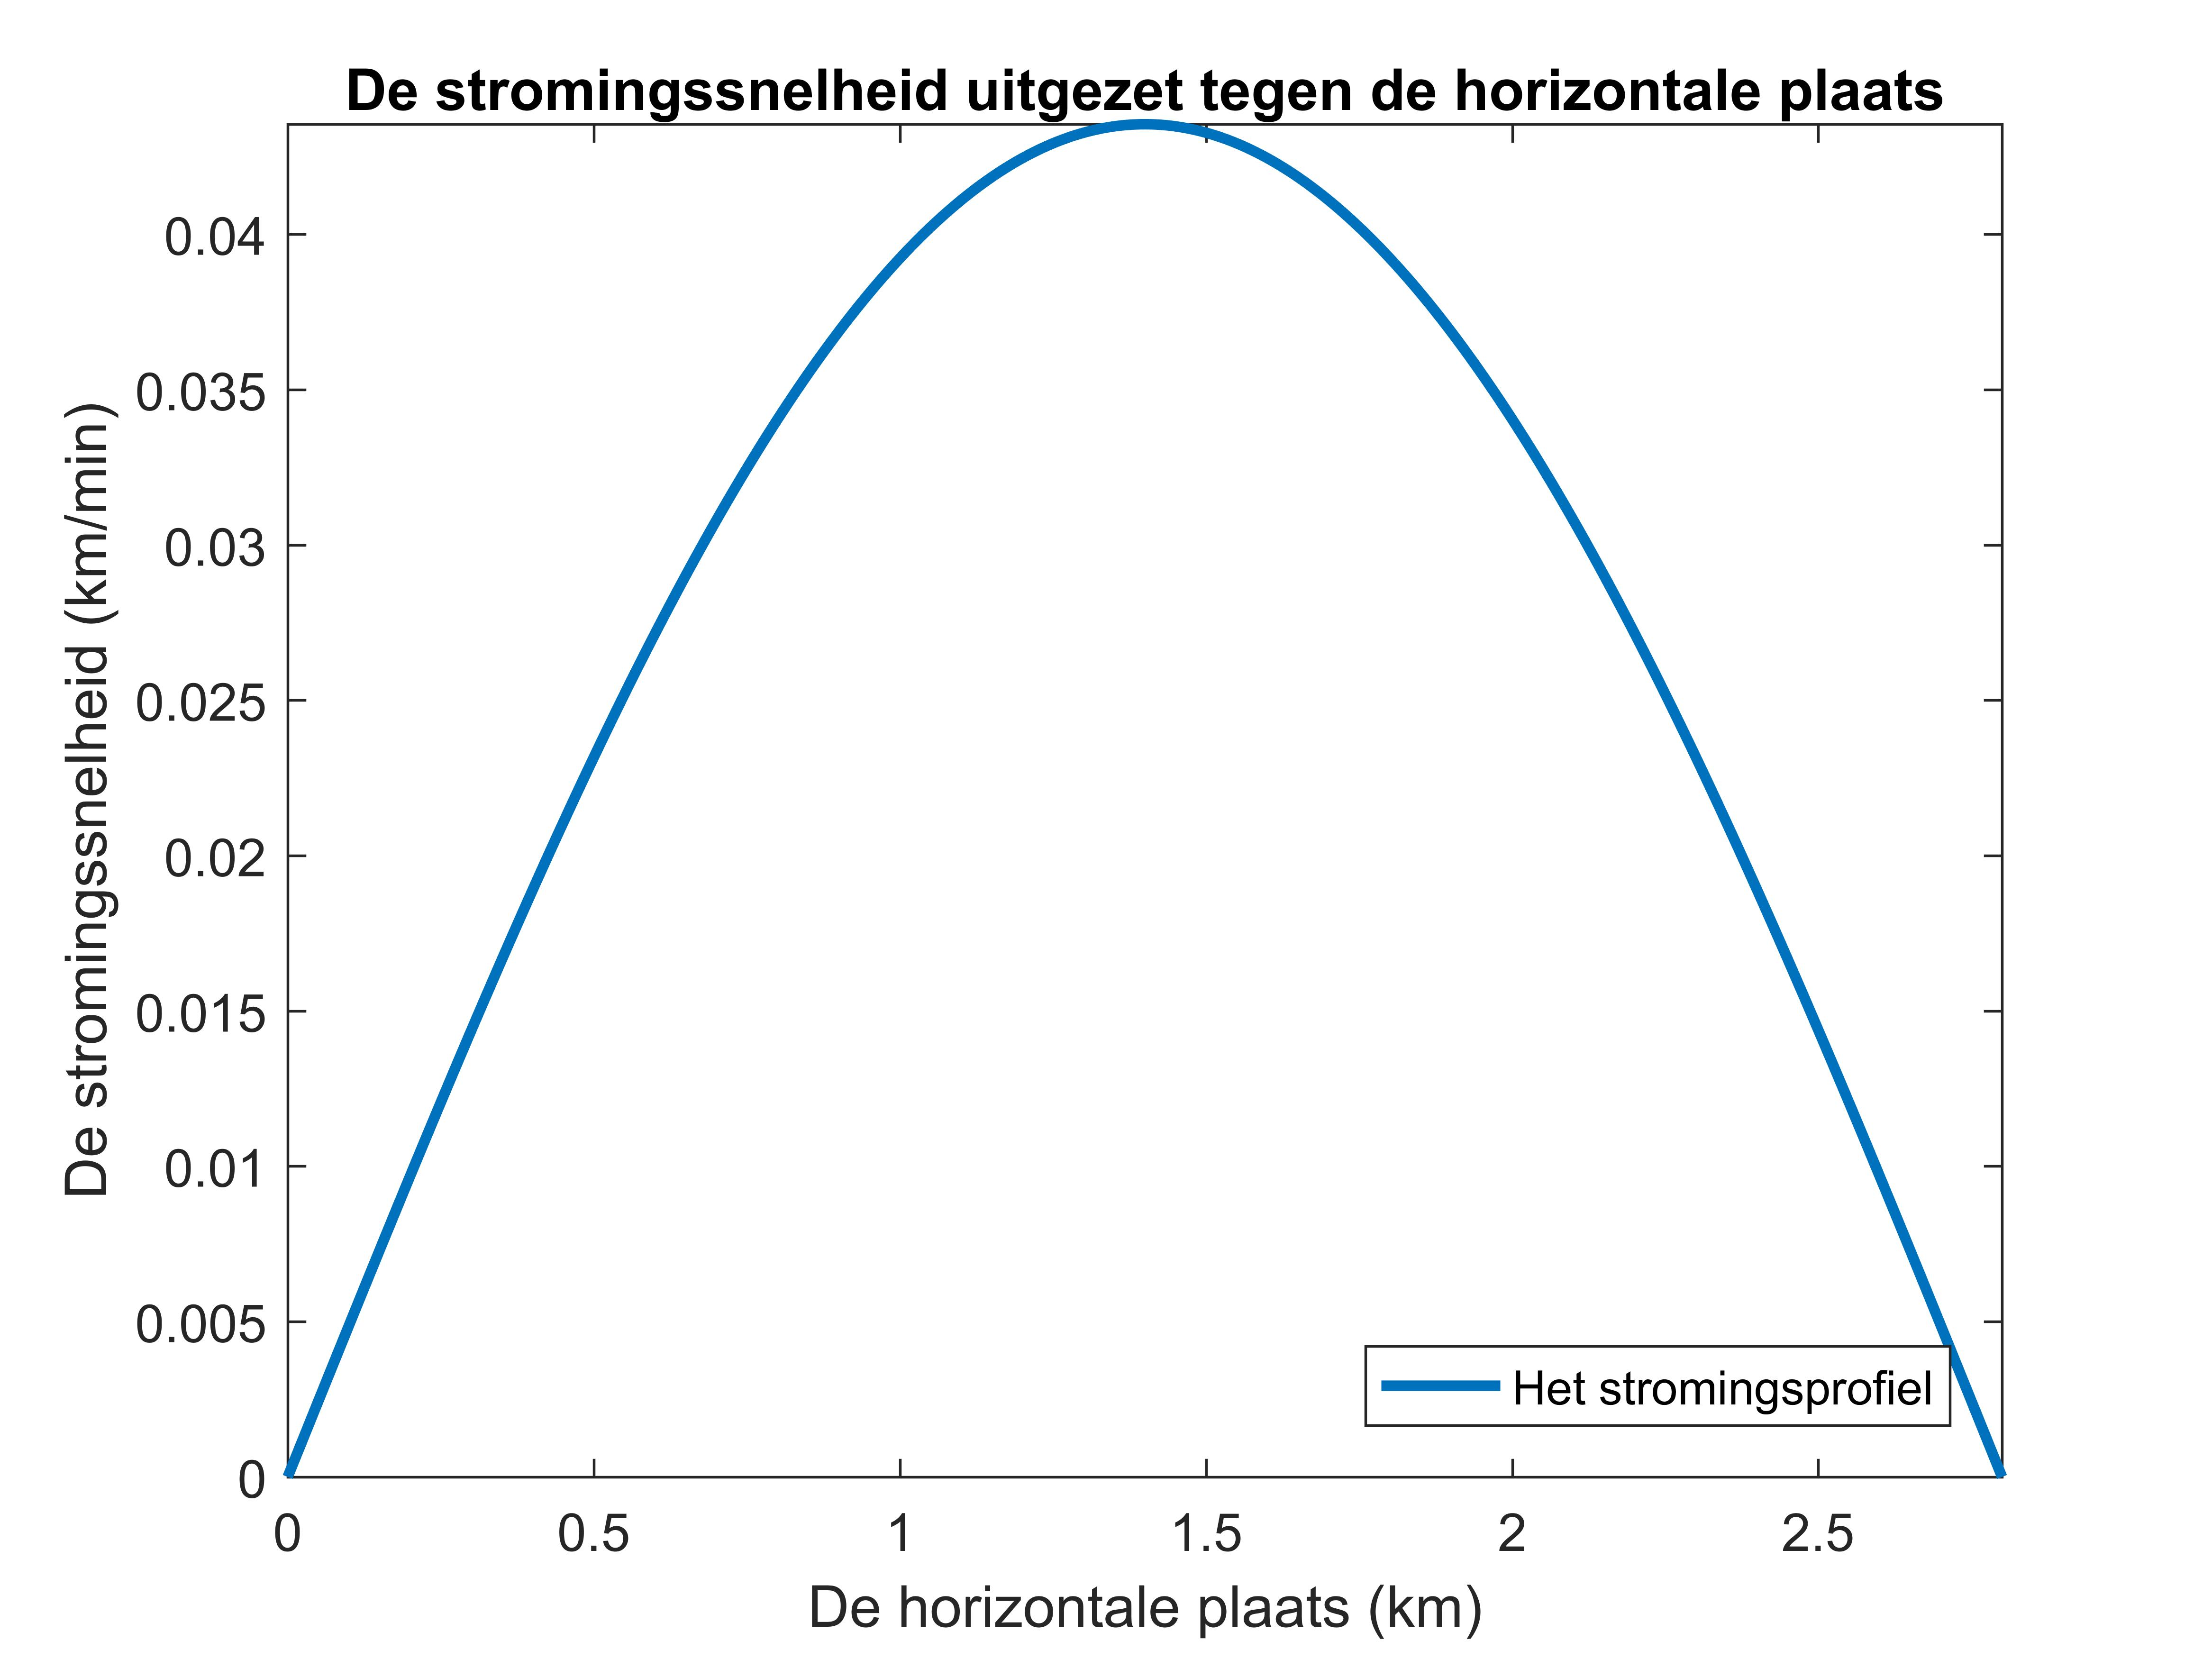
\includegraphics[width=\linewidth]{Sin_stroming_4.jpg}\label{fig:sinstroom}
	\caption{Een mogelijk stromingsprofiel voor de Nijl}
\end{figure}

Door de eerdere eisen in te vullen in MATLAB vinden we voor een boot met een snelheid van \(1~km/min\) een eindtijd van \(T=2.87\) minuten. De resultaten zijn in onderstaande figuren weergegeven.\\
\begin{figure}[H]
	\centering
	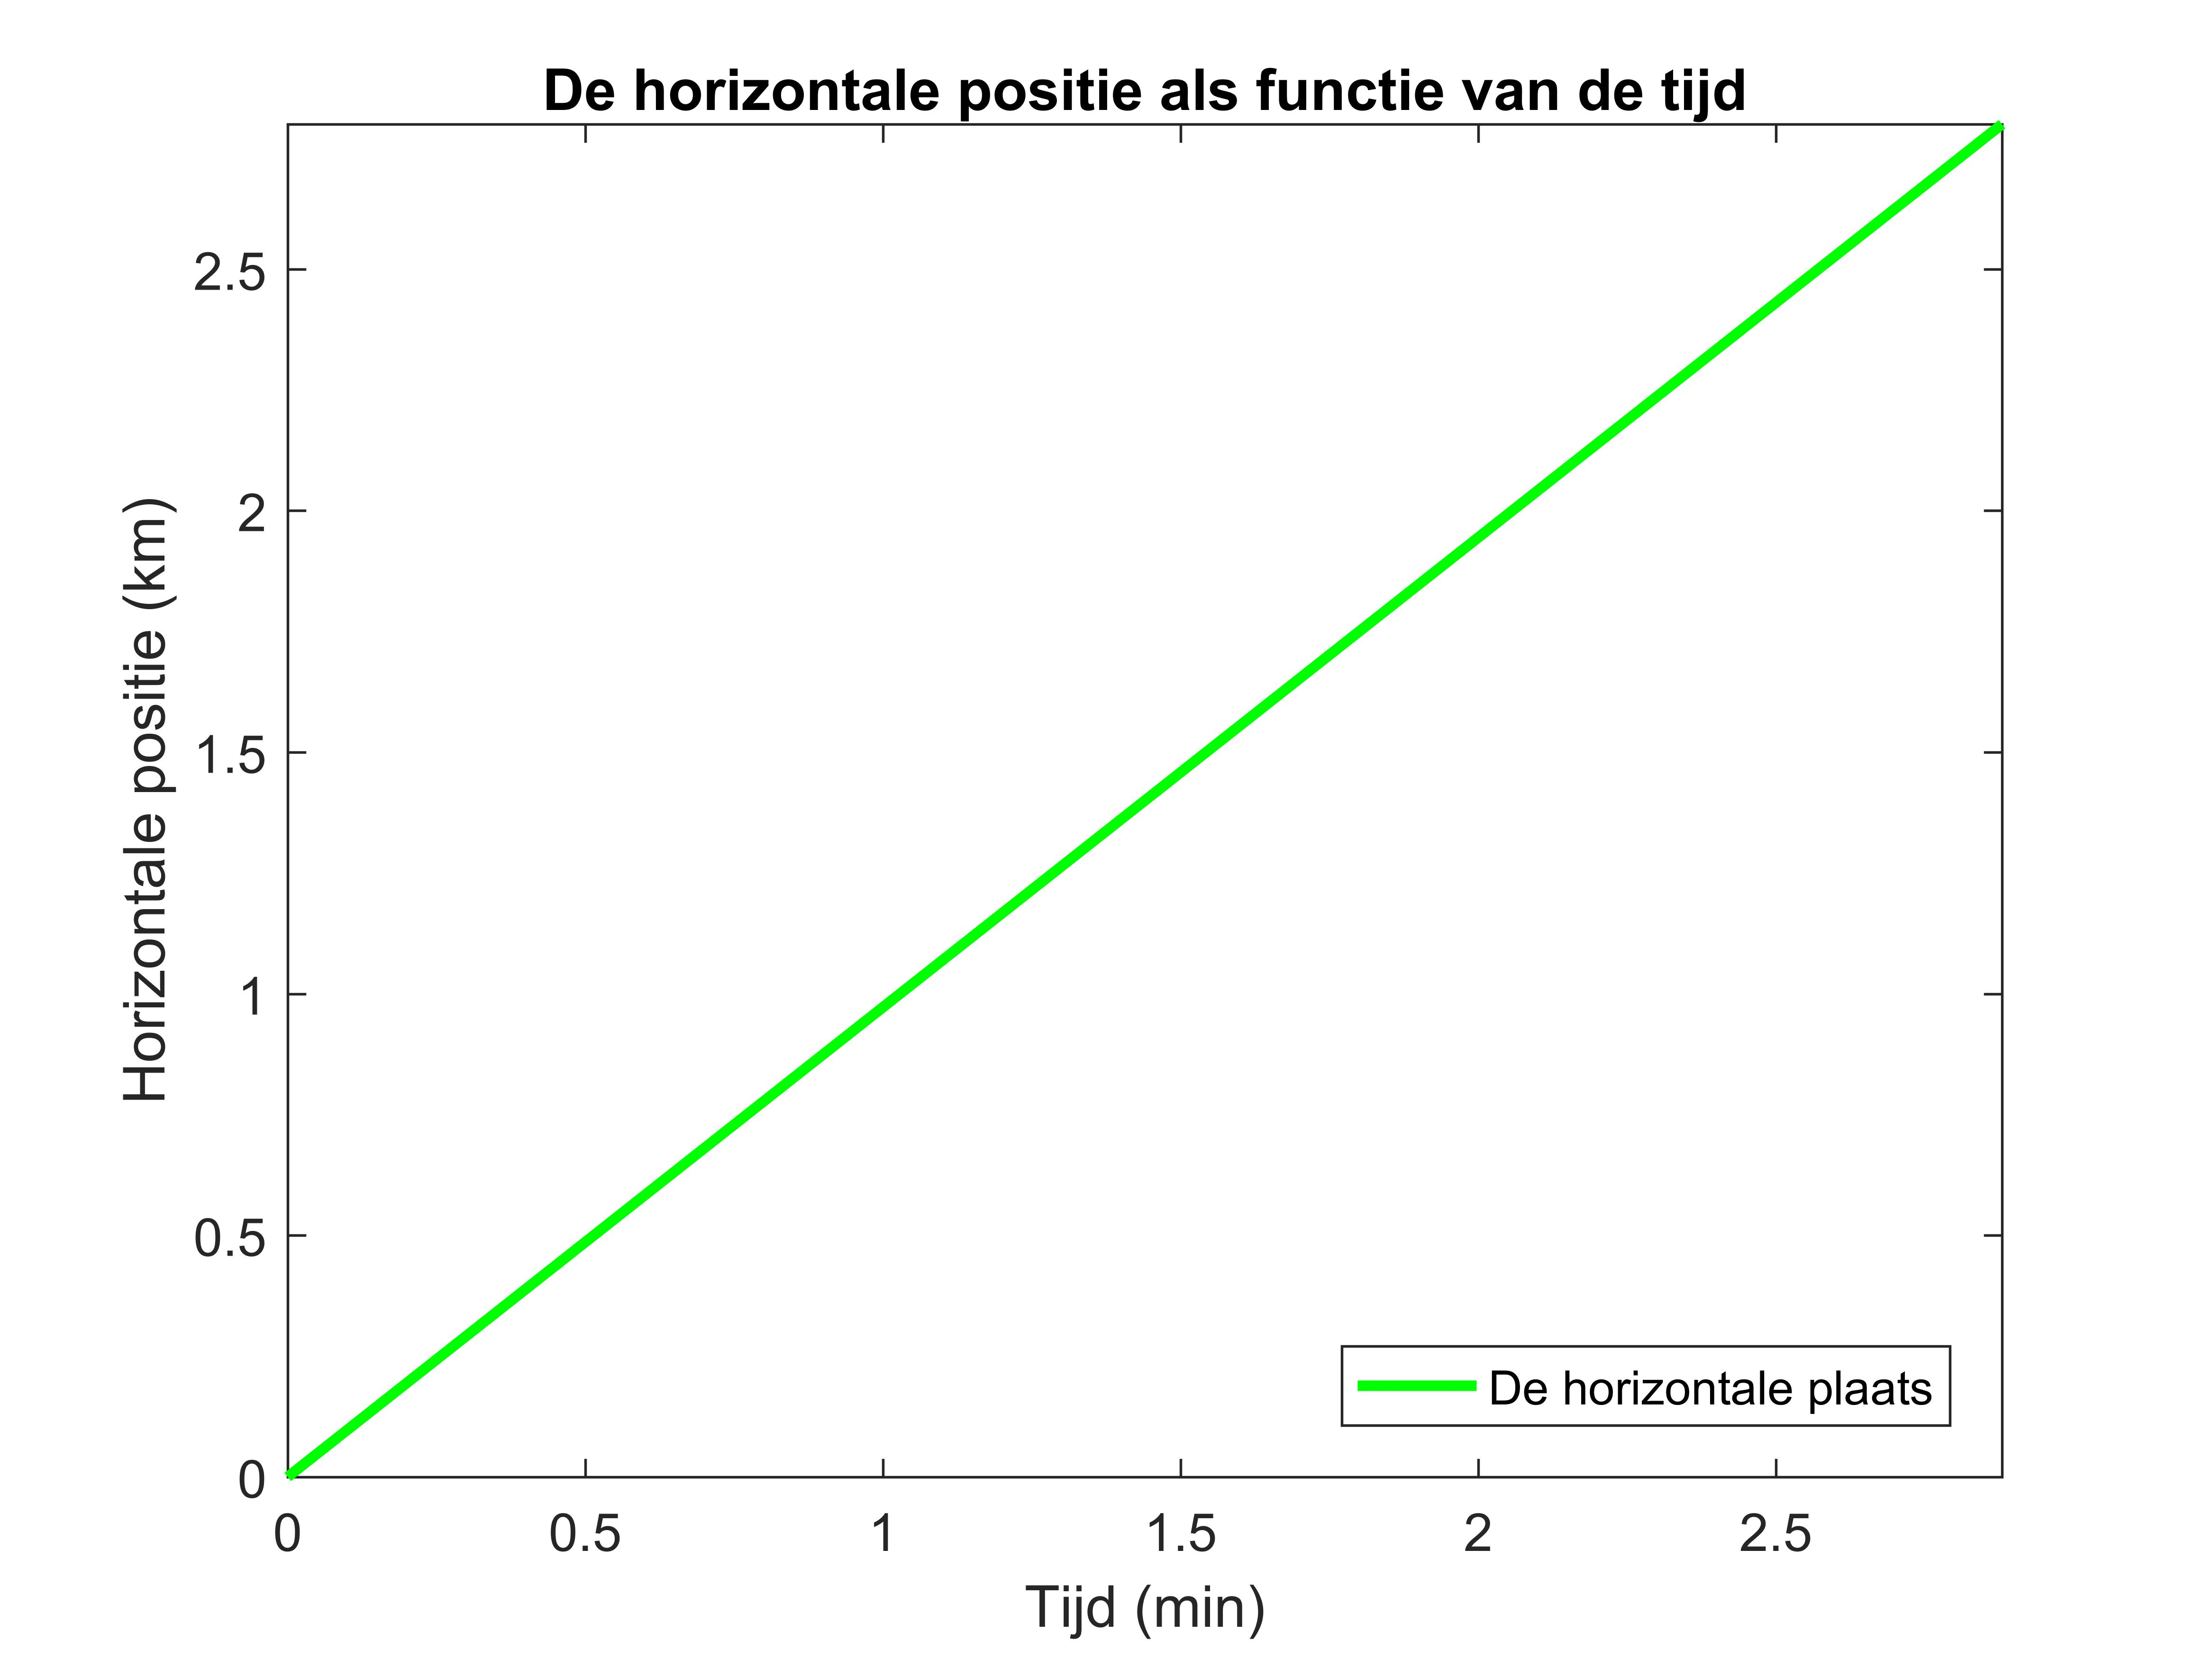
\includegraphics[width=\textwidth]{Sin_xt_3.jpg}
	\caption{De horizontaal positie \(x_1\) uitgezet tegen de tijd \(t\) tijdens een oversteek van de Nijl}\label{fig:sinplots1}
\end{figure}
Figuur \ref{fig:sinplots1} geeft het verband aan tussen de horizontale plaats (de afgelegde afstand ten opzicht van de oever) en de tijd van aankomst bij een punt.
Dit verband is lineair de snelheid in de horizontale richting is dus constant (\(v=\frac{dx_1}{dt}=c\)). \(T=2.87\) en \(x_1(T)=2.8\).
De horizontale snelheid is dus kleiner dan de totale snelheid van de boot.

\begin{figure}[H]
	\centering
	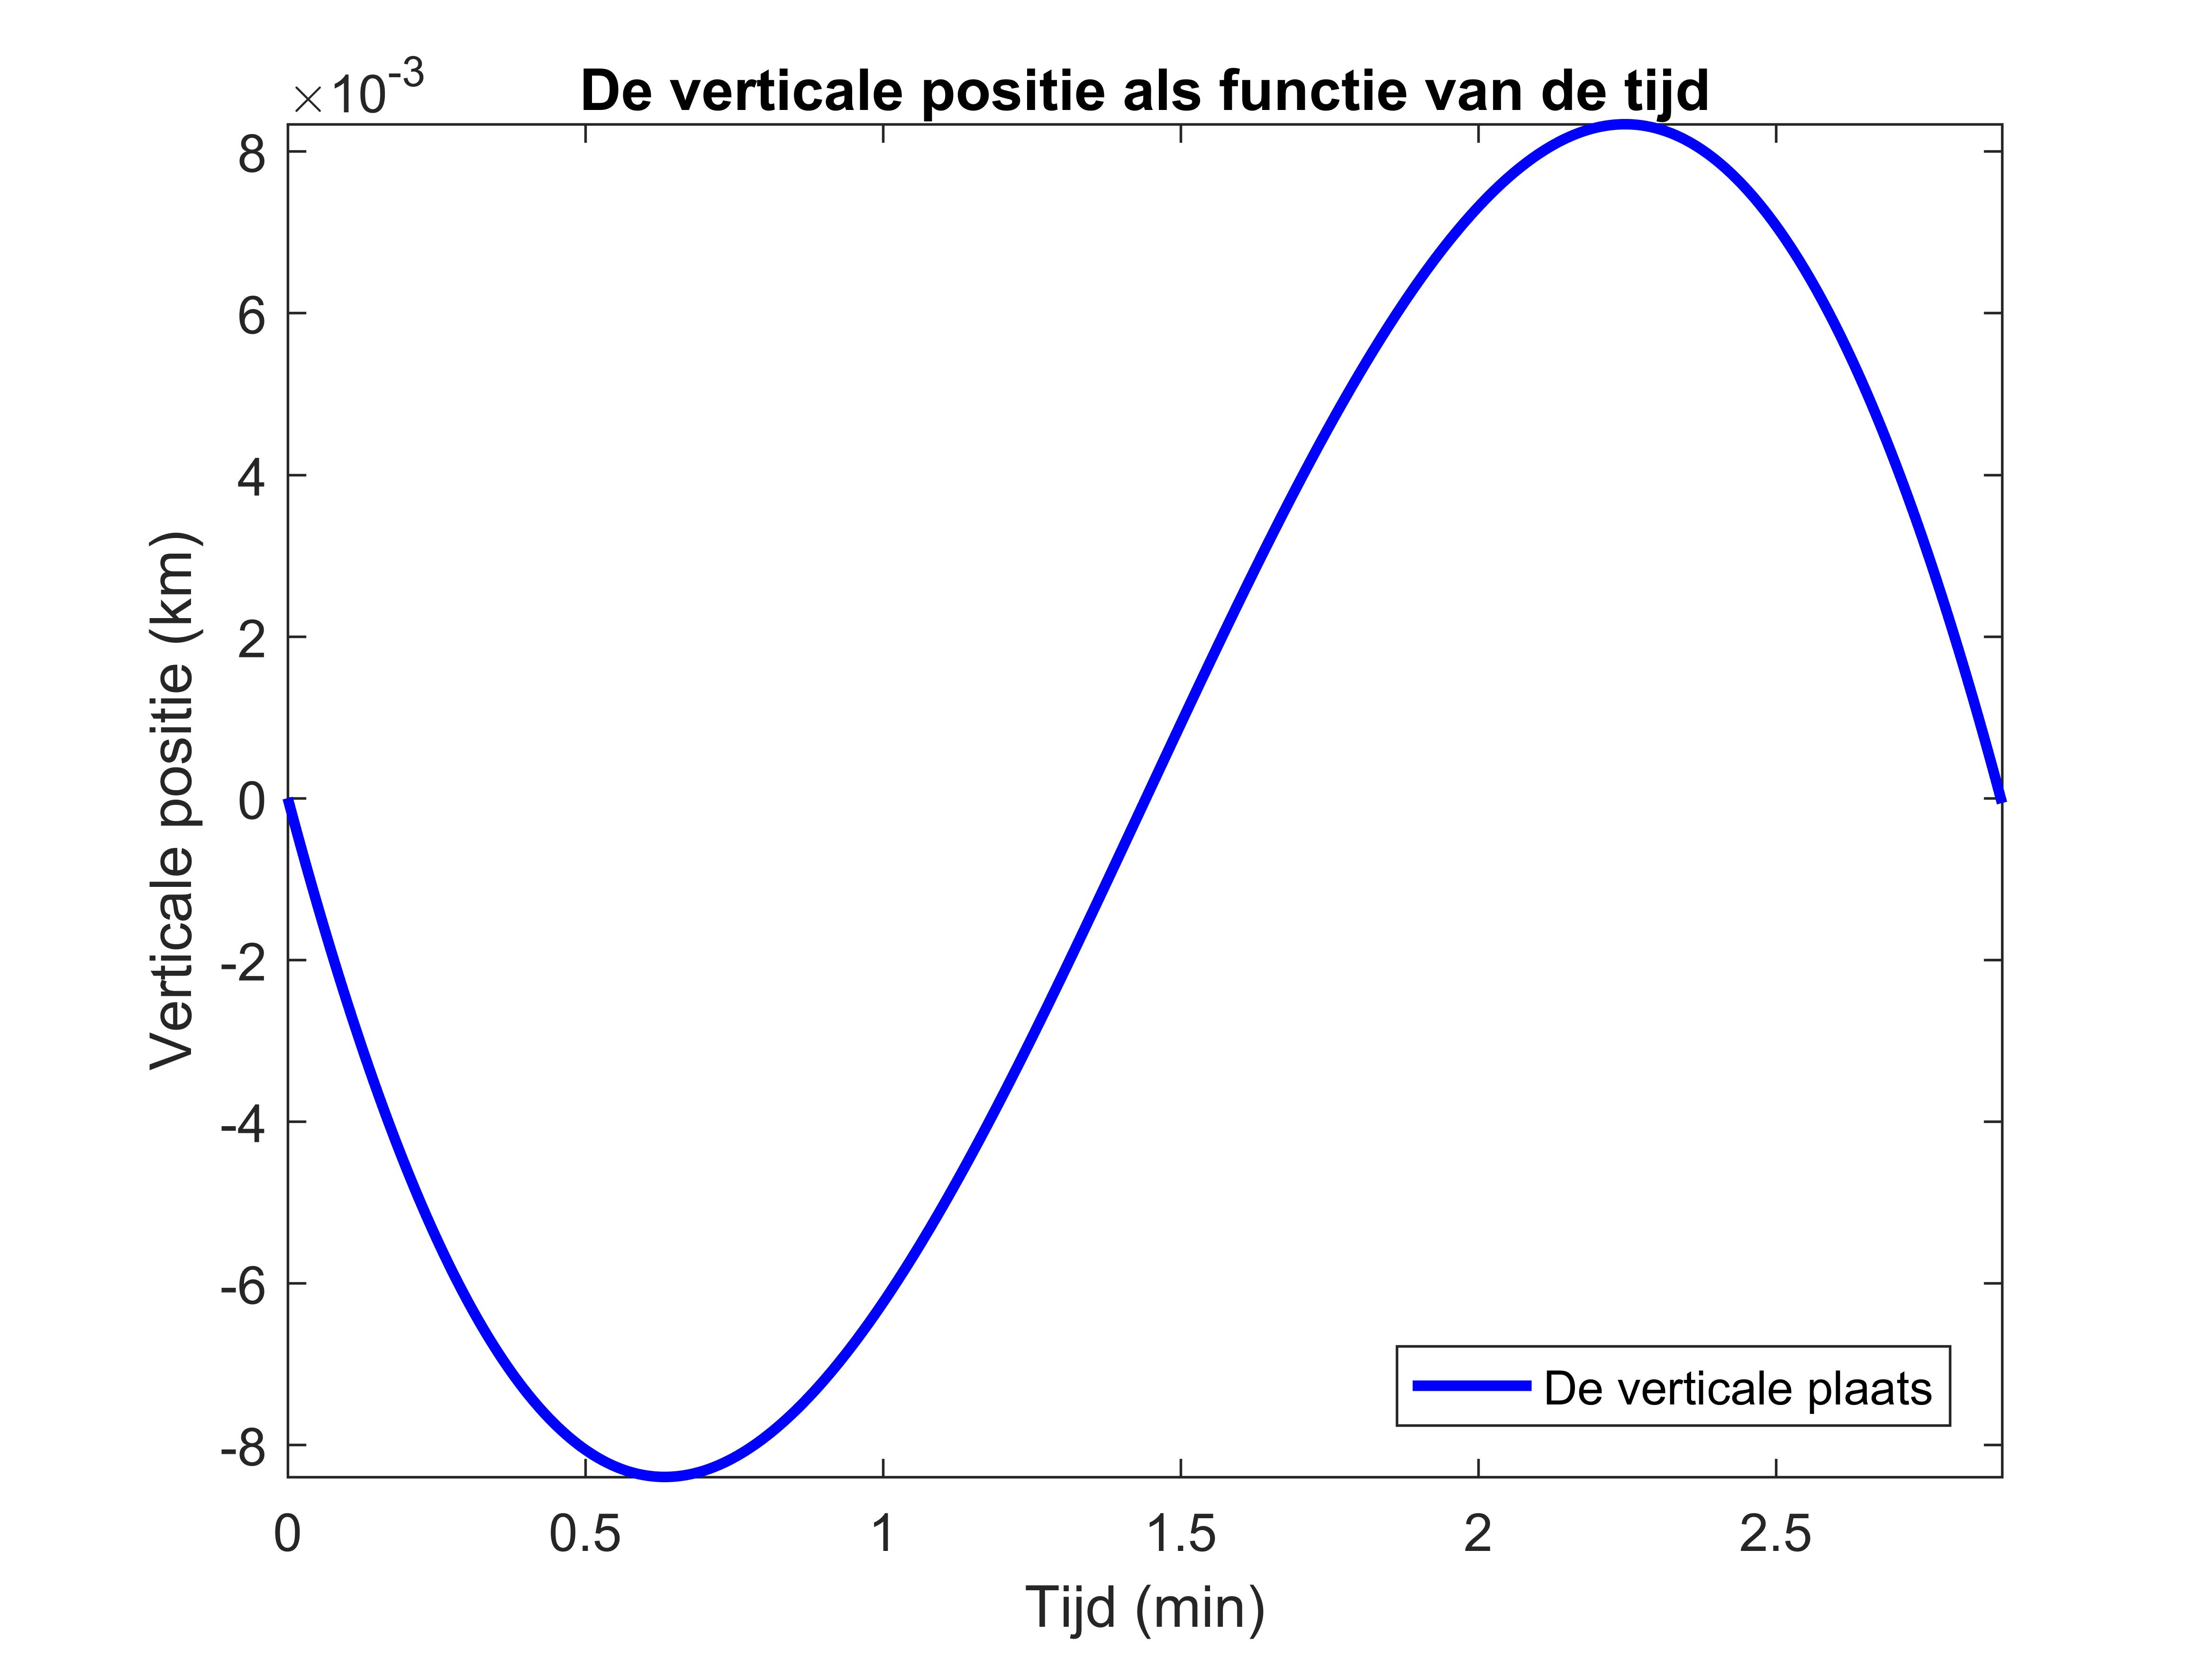
\includegraphics[width=\textwidth]{Sin_yt_2.jpg}
	\caption{De verticale positie \(x_2\) uitgezet tegen de tijd \(t\) tijdens een oversteek van de Nijl}\label{fig:sinplots2}
\end{figure}
Figuur \ref{fig:sinplots2} geeft de verticale plaats aan op een tijdstip \(t\).
Dit verband wordt beschreven door een sinuso\"ide.
De oorzaak hiervan wordt beschreven bij figuur \ref{fig:sinplots3}.
Het is hierbij opmerkelijk dat de verticale positie een hele lage amplitude heeft.
De verticale positie heeft een orde van grootte van \(10^{-3}~km\).
De boot zal tijdens een pad hoogstens 8 meter verwijderd zijn van zijn startpunt (verticaal gezien).

\begin{figure}[H]
	\centering
	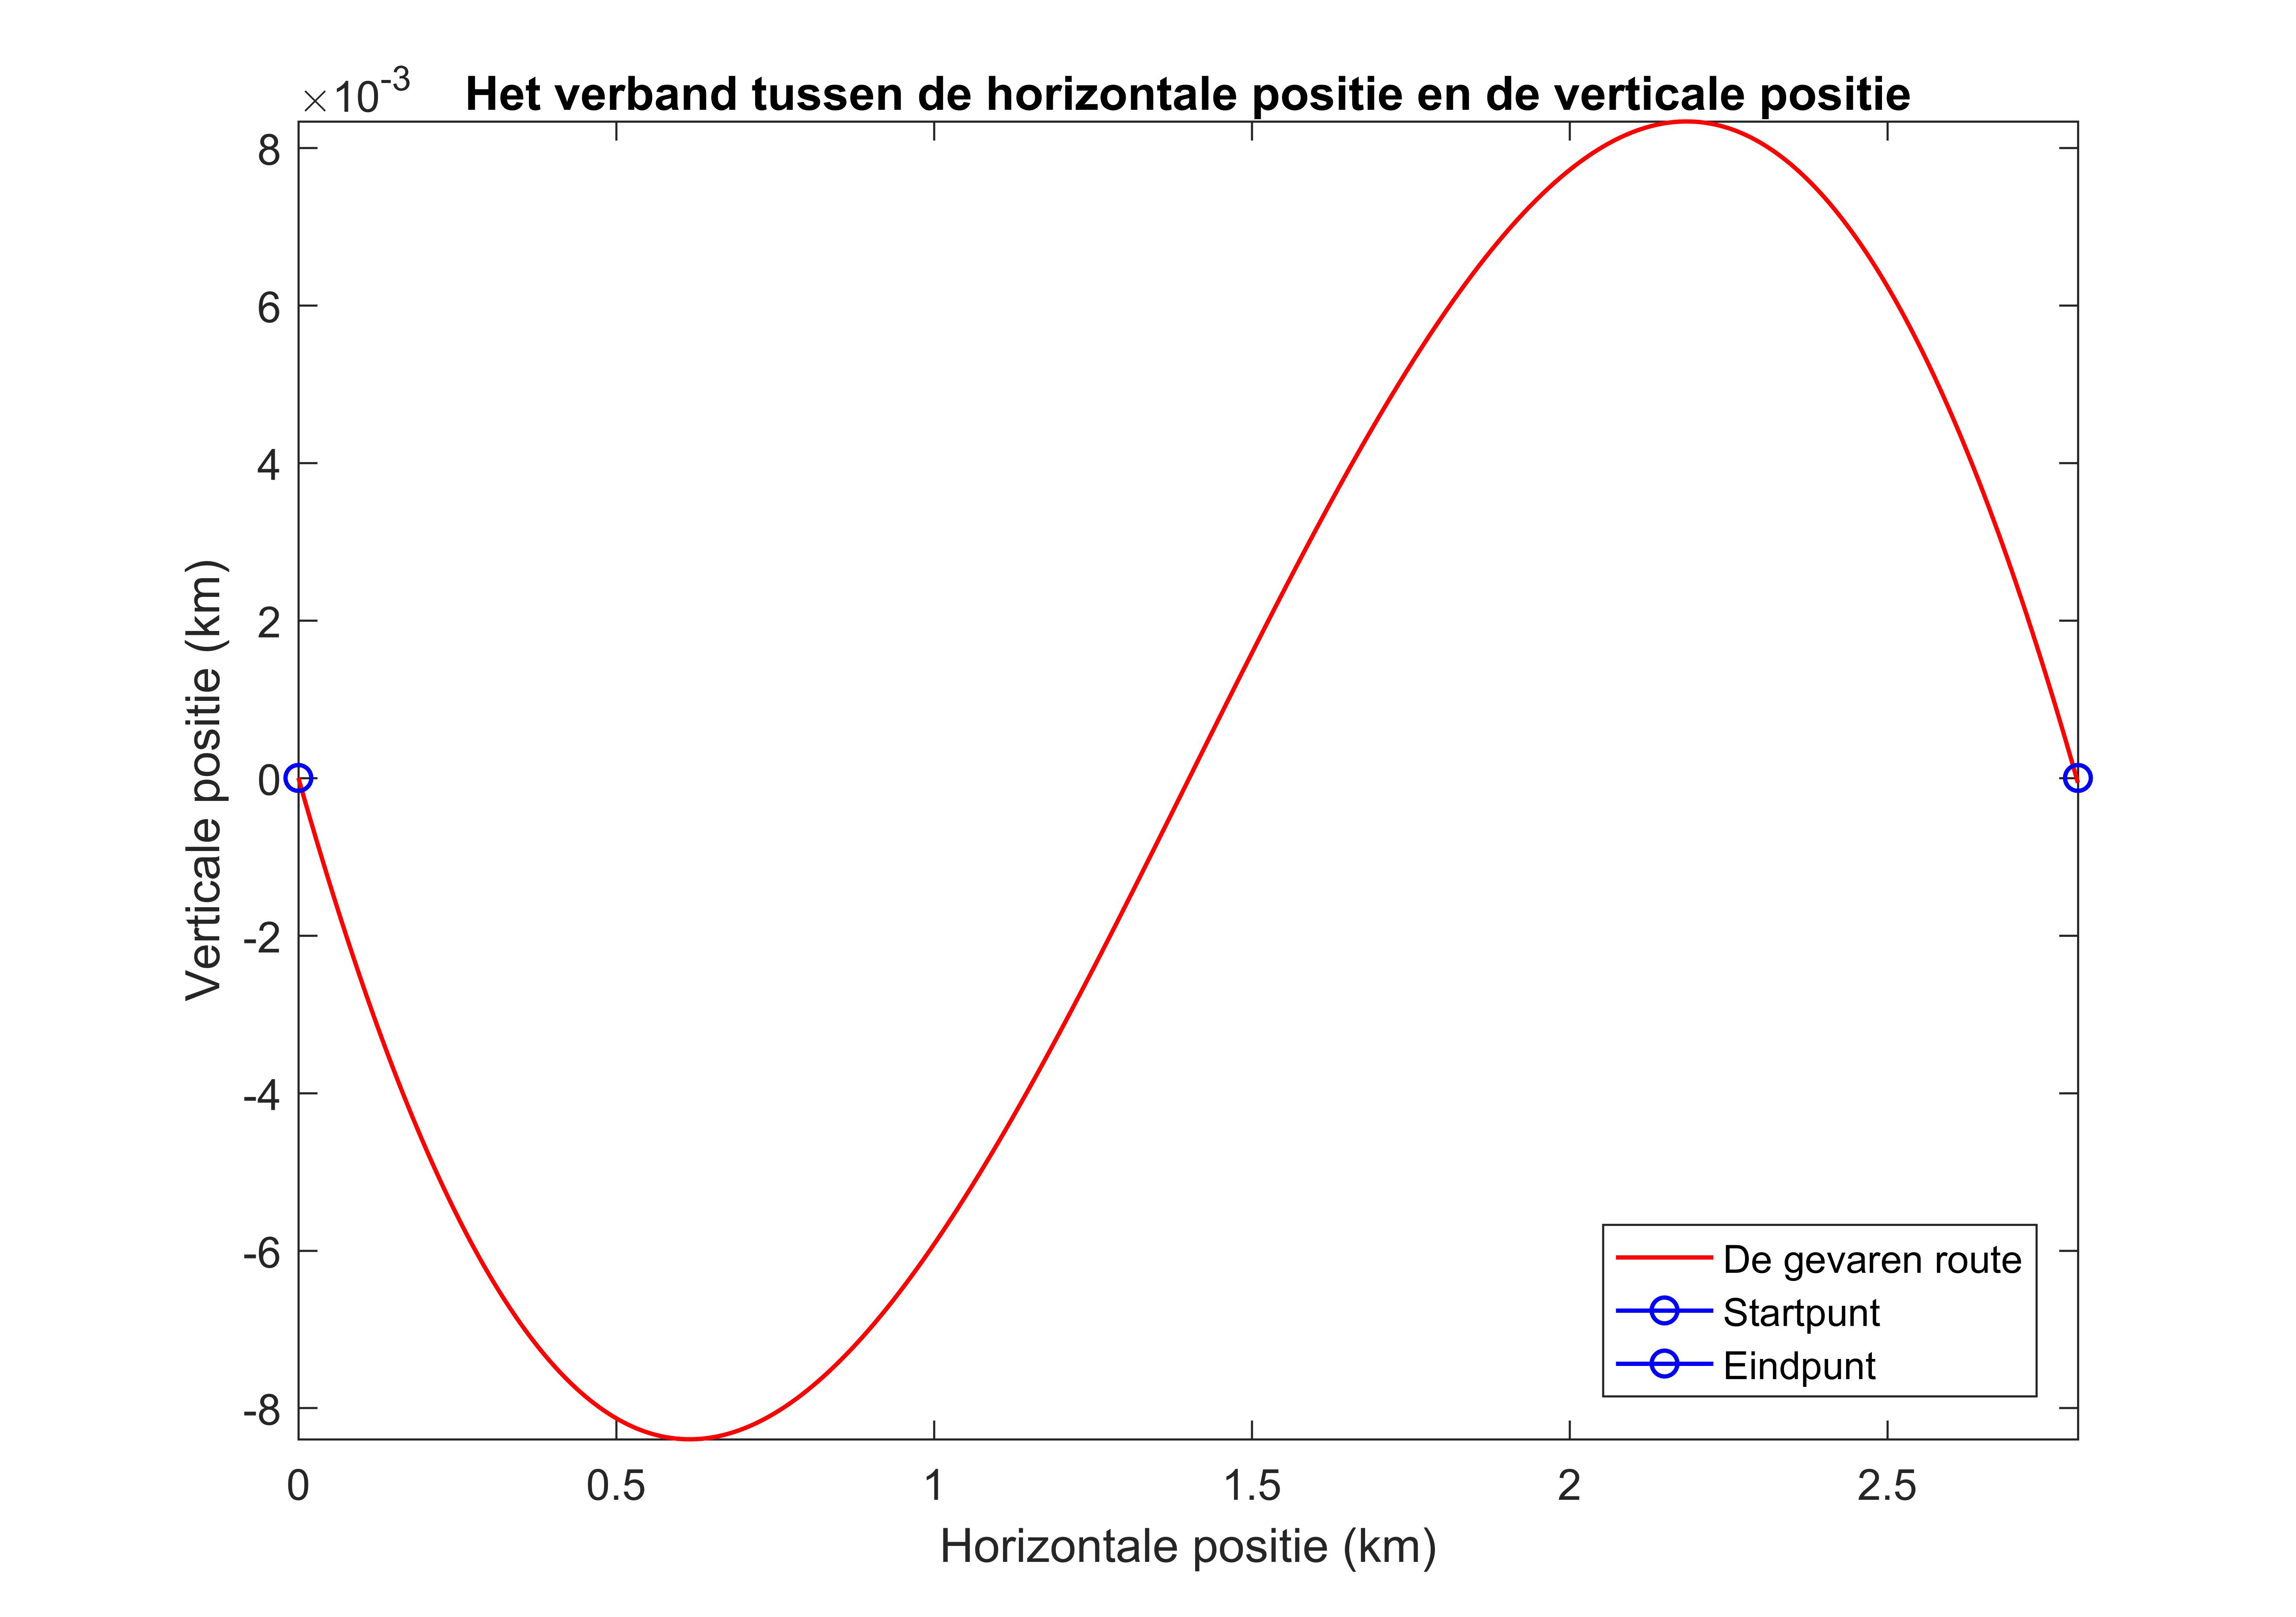
\includegraphics[width=\textwidth]{Sin_xy_2.jpg}
	\caption{Het afgelegde pad tijdens een oversteek van de Nijl}\label{fig:sinplots3}
\end{figure}
Figuur \ref{fig:sinplots3} beschrijft het verloop van een oversteek.
Voor elk tijdstip \(t\) wordt \(x_2(t)\) uitgezet tegen \(x_1(t)\).
Deze vorm beschrijft bijna exact dezelfde sinuso\"ide als de sinuso\"ide gegeven in figuur \ref{fig:sinplots2}.
Dit komt omdat \(x_1(t)\) lineair is ten opzichte van \(t\) en zelfs bijna evenredig: \(x_1(t)= \frac{x_1(T)}{T}t=\frac{2.8}{2.87}t\approx 0.97t\).
De sinuso\"ide vorm kan verklaard worden aan de hand van de stromingsfunctie \(S(x_1)\).
De stroming is zwak aan de oevers en sterk in het midden van de rivier.
Als we dus bij de oevers sterk tegen de stroming invaren, kunnen we in het midden van de rivier deze uitwijking gebruiken als extra versnelling (of minder vertraging).
De daar opgelopen uitwijking stroomafwaarts kan dan weer worden bijgestuurd als de stroming zwak is.
\begin{figure}[H]
	\centering
	\includegraphics[width=\textwidth]{Sin_stuur_4.jpg}
	\caption{De stuurhoek uitgezet tegen de tijd tijdens een oversteek van de Nijl}\label{fig:sinplots4}
\end{figure}
Tot slot wordt in figuur \ref{fig:sinplots4} de stuurhoek uitgezet tegen de tijd.
De stuurhoek is overal negatief, en het sterkst negatief in het midden van de rivier.
Als de stroming het sterkst is, draait de boot dus sterk bij om zijn richting voldoende bij te draaien, zodat hij met een maximale snelheid richting het eindpunt kan varen als de stroming zwakker is.\\

Deze plots zijn allemaal bepaald voor een boot met een snelheid van \(1~km/min\).
Onze boot heeft echter geen snelheid van \(1~km/min\) maar \(0.63~km/min\) Onze boot zal er dus in totaal \(\frac{T}{0.63}=4.57\)minuten over doen.


	\chapter{Minimaliseren van kosten}\label{sec:laagsteKosten}
Waar het eerste model een constante snelheid aannam laten we in dit model de snelheid varieren afhankelijk van een stuwkracht die in de richting waarin de boot vaart wordt gezet. Dit betekent dat de staat van een bootje niet alleen meer bepaald is door diens locatie maar ook door diens snelheid. Ook is er een extra variabele waarmee gestuurd kan worden: de stuwkracht.

De kosten van een reis worden in dit model bepaald door de som van de verbruikte tijd en de verbruikte energie. We defini\"eren we een kostenfunctie \(C(t)\) die de kosten tot een bepaald tijdstip aangeeft.
	\begin{align}
		C(t) = at +(1-a)E(t)
	\end{align}
Hier geeft \(E(t)\) de totaal verbruikte energie op tijdstip \(t\) aan, \(a\in[0,1]\) is een te kiezen constante die de verhouding tussen de kosten van energie en de kosten van tijd aangeeft. Wederom is \(T\) het tijdstip van aankomst en dus willen we \(C(T)\) minimaliseren. Merk op dat voor \(a = 1\) de te minimaliseren kotsen functie gelijk is aan de functie die we minimaliseerden in de voorgaande hoofdstukken.

\section{Enkele eisen}
We stellen enkele randvoorwaarden bovenop de randvoorwaarden van het eerste model:
\begin{itemize}
	\item[] \(v(0) = v(T) = 0\). Dit is van toepassing bij het oversteken van een rivier: De boot moet eerst vaart maken en niet tegen de tegenoverstaande wal botsen.
	\item[] Tot slot stellen we dat \(v(t) \geq 0:\forall t \in \mathbb{R}_{\geq 0}\). Dit omdat er voor enigzins realistische stromingen niet van het doel afgevaren moet worden in een goedkoopste oplossing.
\end{itemize}

\section{Schrijven als integraal}
Om de kostenfunctie \(C(T)\) te minimaliseren met gebruik van de hamiltoniaanstelling moeten we wederom onze functie als integraal van \(0\) tot \(T\) schrijven.

Allereerst vinden we een bruikbare vorm van \(E(T)\). 
We beschouwen de totale hoeveelheid energie als de verrichte arbeid \(W\) over het traject dat de boot aflegt. Dit traject noemen we \(\mathcal{C}\). 
Voor \( \mathcal{C} \) hebben we een parametrisatie \( \mathbf{f}: [0, T] \rightarrow \mathcal{C},~t \mapsto (x(t), y(t)) \) met afgeleide $ f^\prime(t) = (x^\prime(t), y^\prime(t)) $. 
Verder heeft $ \mathcal{C} $ een ori\"entatie $ \mathbf{\tau} $ waar deze parametrisatie bij past. Laat $ F_{x_1} $ en $ F_{x_2} $ de componenten van $ F $ in respectievelijk de $ x_1 $- en $ x_2 $-richting zijn. 
Dan geldt voor de arbeid de eigenschap:
\begin{align*}
		W &= \int_\mathcal{C} \langle \mathbf{F}, \mathbf{\tau} \rangle dq \\
		&= \int_\mathcal{C} F_{x_1} dx_1 + F_{x_2} dx_2
\end{align*}
\(F\) is zoals gebruikelijk de geleverde kracht van de boot.\\
Ook geldt:
\begin{align*}
		v_{x_1} &= \frac{dx_1}{dt} & v_{x_2} &= \frac{dx_2}{dt}
\end{align*}
Met toepassing van de substitutiemethode volgt nu:
\begin{align*}
	dx_1 &= v_{x_1}dt & dx_2 &= v_{x_2}dt\\
\end{align*}
en
\begin{align*}
	W = \int_\mathcal{C} F_{x_1} dx_1 + F_{x_2} dx_2 &= \int_0^T F_{x_1} v_{x_1} + F_{x_2} v_{x_2} \, dt\\
	&= \int_0^T \langle \mathbf{F}, \mathbf{v} \rangle \, dt
\end{align*}
Omdat in ons model \( \mathbf{F} \) en $ \mathbf{v} $ dezelfde richting hebben, geldt $ \langle \mathbf{F}, \mathbf{v} \rangle = \Vert \mathbf{F} \Vert \Vert \mathbf{v} \Vert $. Als we nu $ F $ schrijven voor $ \Vert \mathbf{F} \Vert $ en $ v $ voor $ \Vert \mathbf{v} \Vert $ , vinden we, omdat \(W=E(T)\), dat:
\begin{align}
	E(T) &= \int_0^T \langle \mathbf{F}, \mathbf{v} \rangle \, dt\\
	&= \int_0^T \Vert \mathbf{F} \Vert \Vert \mathbf{v} \Vert \, dt\\
	&= \int_{0}^{T} v(t)F(t) dt\label{eq:E(T)int}
\end{align}
Hierbij geeft \(v(t)\) de snelheid van de boot op tijdstip \(t\) aan en \(F(t)\) de geleverde kracht op tijdstip \(t\). Verder geldt de bekende integraal:
\begin{align}
	T &= \int_{0}^{T} dt.\label{eq:T-energ}
\end{align}
Met \eqref{eq:E(T)int} en \eqref{eq:T-energ} zijn we nu in staat om een integraal voor \(C\) op te stellen afhankelijk van \(T\):
\begin{align*}
	C(T) = a T + (1 - a) E(T) = a \int_{0}^{T} dt + (1-a)\int_0^T F v dt 
\end{align*}
Voor \(C(T)\) vinden we dus de uitdrukking:
\begin{align}
	C(T)=\int_0^T a + (1-a)F(t)v(t) dt\label{eq:Cint}
\end{align}

\section{Nieuwe hamiltoniaan opstellen}
Omdat \(C(T)\) nu als integraal guitgedrukt is en de begin- en eindvoorwaarden bepaald zijn kan \(C(T)\) door middel van de Hamiltoniaanstelling geoptimaliseerd worden. Analoog aan sectie \ref{sec:Hamilton1} worden de afgeleiden voor \(x_1\) en \(x_2\) opgesteld. Omdat de snelheid nu echter niet constant is wordt deze ook meegenomen in de afgeleiden.
\begin{align}
	x_1^\prime &= v \cos(u(t)) \label{eq:x1'kosten}\\ 
 	x_2^\prime &= v \sin(u(t)) + S(x_1)\label{eq:x2'kosten}
\end{align}
Om \(v^\prime\) te bepalen defini\"eren we eerst \(\widetilde{F}\), de som van alle werkende krachten op de boot. De tweede wet van Newton stelt
\begin{align*}
	\widetilde{F} = m v^\prime
\end{align*}
In dit model worden alleen de door de boot geleverde kracht \(F\) en de wrijvingskracht \(F_w(v)\) in de berekeningen opgenomen. \(\widetilde{F}\) wordt gegeven als de som van deze twee krachten
\begin{align*}
	\widetilde{F}= F+ F_w(v)
\end{align*}
en dus geldt
\begin{align}
v^\prime   = \frac{F + F_w(v)}{m}. \label{eq:v'}
\end{align}\\
Nu alle afgeleiden en randvoorwaarden bekend zijn kan de Hamiltoniaan \(H_2\) worden opgesteld.
\begin{align*}
	H_2(x_1,x_2,v,\lambda_1,\lambda_2,\lambda_3,F,u) &= \lambda_1  x_1^\prime(t) + \lambda_2 x_2^\prime(t)+ \lambda_3 v^\prime(t) + f(x_1,x_2,v,F,u)
\end{align*}
Specifiek wordt deze gegeven door
\begin{align*}
H_2 = \lambda_1v\cos(u)+\lambda_2(v\sin(u)+ S(x_1)) + \lambda_3\frac{(F+F_w (v))}{m} + (1-a)Fv + a
\end{align*}
Met de voorwaardes
\begin{align*}
	x_1(0) = 0 && x_1(T) &= {x_1}_T\\
	x_2(0) = 0 && x_2(T) &= {x_2}_T\\
	v(0) = 0 && v(T) &= 0
\end{align*}

\section{Hamiltoniaanstelling gebruiken}
Met behulp van de zojuist opgestelde hamiltoniaan bepalen we de afgeleiden van de schaduwvariabelen \(\lambda_1, \lambda_2\) en \(\lambda_3\).
\begin{align}
	\lambda_1^\prime = -\frac{\partial H_2}{\partial x_1} &= -\lambda_2 S^\prime(x_1)\label{eq:lambda1'} \\ 
	\lambda_2^\prime = -\frac{\partial H_2}{\partial x_2} & = 0 \label{eq:lambda2'}\\ 
	\lambda_3^\prime = -\frac{\partial H_2}{\partial v} &= -(\lambda_1 \cos(u)+\lambda_2 \sin (u) +\lambda_3 \frac{F_w^\prime(v)}{m} +(1-a)F) \label{eq:lambda3'}\\
\end{align}
Volgens de Hamiltoniaanstelling geldt bij een minimale \(C(T)\) dat
\begin{align}
	0 = \frac{\partial H_2}{\partial u} &= -\lambda_1 v \sin(u)+\lambda_2 v \cos(u)\label{eq:dH/du}\\ 
	0 =	\frac{\partial H_2}{\partial F} &= \frac{\lambda_3}{m} + (1-a)v \label{eq:dH/dF}
\end{align}

\section{Eliminatie en vereenvoudigen van de afgeleiden}
Door analytische manipulaties kunnen deze vergelijkingen gereduceerd worden tot slechts vier afgeleiden.
\subsection{Eliminatie van Sinus en Cosinus en \(u\)}		
Vegelijking \eqref{eq:dH/du} geeft
	\begin{align*}
	0 = v(-\lambda_1\sin(u) + \lambda_2 \cos(u))
\end{align*}
dus \(v=0\) of
\begin{align*}
	\lambda_1 \sin(u) = \lambda_2\cos(u).
\end{align*}
Dit probleem is identiek het probleem beschreven in \ref{sec:Eliminatie van u} en kent daarom ook dezelfde oplossingen zijnde:
\begin{align}
	\sin(u) = \frac{\mu}{\sqrt{1+\mu^2}} &&
	\cos(u) = \frac{1}{\sqrt{1+\mu^2}} \label{eq:Coswaarde}
\end{align} 

\subsection{Eliminatie van \(F, F_w(v),\lambda_3\) en \(v\)}
Uit vergelijking \eqref{eq:dH/dF} volgt
\begin{equation}
	\lambda_3=-(1-a)mv \label{eq:l3=-v}
\end{equation}
dus
\begin{align}
	\lambda_3^\prime =-(1-a)mv^\prime. \label{eq:l3'=-v'}
\end{align}
Invullen van vergelijkingen \eqref{eq:v'} en \eqref{eq:lambda3'} in vergelijking \eqref{eq:l3'=-v'} geeft nu
\begin{align*}
	(1-a)m\frac{F + F_w(v)}{m} = \lambda_1 \cos(u)+\lambda_2 \sin (u) +\lambda_3 \frac{F_w^\prime (v)}{m} +(1-a)F.
\end{align*} 
Invullen van vergelijking \eqref{eq:l3=-v} geeft
\begin{align*}
	(1-a)F + (1-a)F_w(v) = \lambda_1 \cos(u)+\lambda_2 \sin (u) -(1-a)mv\frac{F_w^\prime (v)}{m} +(1-a)F
\end{align*}	  
dus voor \(v\neq 0\) geldt nu
\begin{align*}
	(1-a)F_w(v) &= \lambda_1 \frac{1}{\sqrt{1+\mu^2}}+\lambda_2 \frac{\mu}{\sqrt{1+\mu^2}} -(1-a)v F_w^\prime (v)\\
	(1-a)(F_w(v) + v F_w^\prime (v)) &= (\lambda_1+\lambda_2\mu)\frac{1}{\sqrt{1+ \mu^2}}\\
	F_w(v) + v F_w^\prime (v) &= \lambda_1 \frac{1+\mu^2}{\sqrt{1+\mu^2}}~\frac{1}{1-a}
\end{align*}
Voor \(F_w (v)\) kiezen we
\begin{align}
	F_w (v) = -cv^2.
\end{align}	 
Hier is \(c>0\) de wrijvingsconstante. Nu geldt:
\begin{align}
	F_w^\prime (v) = -2cv.
\end{align}
Invullen in de eerdere gelijkheid geeft
\begin{align*}
	-cv^2 + v(-2cv) &= \lambda_1\frac{\sqrt{1+\mu^2}}{1-a}\\
	-3cv^2 &= \lambda_1\frac{\sqrt{1+\mu^2}}{1-a}.
\end{align*}
We vinden dus een uitdrukking voor \(v\) in \(\lambda_1\),  \(\mu\) en de constanten \(a\) en \(c\):
\begin{equation}
	v = \sqrt{\frac{-\lambda_1\sqrt{1+\mu^2}}{3c\cdot(1-a)}} \label{eq:Vwaarde}
\end{equation}

\subsection{Invullen van de gelijkheden}
Nu blijven enkel de volgende vergelijkingen over:
\begin{align*}
	x_1^\prime &= v \cos(u)\\
	x_2^\prime &= v \sin(u) + S(x_1)\\
	\lambda_1^\prime &= -\lambda_2 S^\prime(x_1)\\
	\lambda_2^\prime &= 0
\end{align*}
Met de gevonden gelijkheden \eqref{eq:Coswaarde} en \eqref{eq:Vwaarde} reduceren deze vergelijkingen zich verder tot:
\begin{align}
	x_1^\prime &= \sqrt{\frac{-\lambda_1}{3c\cdot(1-a)\sqrt{1+\mu^2}}} \\
	x_2^\prime &= \mu \sqrt{\frac{-\lambda_1}{3c \cdot (1-a)\sqrt{1+\mu^2}}} +S(x_1) \\
	\lambda_1^\prime &= -\lambda_2 S^\prime(x_1)\\
	\lambda_2^\prime &= 0
\end{align}
met de eisen:
\begin{align*}
	x_1(0) = 0 && x_1(T) &= {x_1}_T\\
	x_2(0) = 0  && x_2(T) &= {x_2}_T
\end{align*}

	
	\chapter{Discussie}
Ons onderzoek kenmerkte zich door de wiskundige focus die we gebruikten om het probleem te modelleren. We losten de problemen eerst grotendeels analytisch op om de rekentijd die de computer nodig zou had te minimaliseren. Met deze aanpak is het mogelijk om relatief complexe problemen in een korte tijd door te rekenen. De precisie van dit rekenwerk is zeer hoog.

Om dit onderzoek grotendeels analytisch te kunnen doen kent ons model een aantal grote versimpelingen ten opzichte van de werkelijkheid. Zo werken wij met een enkele wrijvingsterm welke afhankt van de snelheid om alle wrijvingsfactoren samen te vatten. Ook gaan we er van uit dat de boot in zeer korte tijd scherpe hoeken kan draaien, een onbeperkte hoeveelheid brandstof bij zich draagt en dat het gewicht van de boot niet verandert ondanks dat er brandstof verbruikt wordt. Op de boot na gaan we uit van een volledig constant systeem en de stroming varieert enkel in de \(x_1\) richting.

Met meer tijd hadden we graag de code voor het vinden van een numerieke oplossing voor de goedkoopste route afgerond. Het zou ook interresant zijn om het model uit te breiden naar stromingsprofielen welke niet alleen in de \(x_1\) richting veranderen maar ook in de \(x_2\) richting. 

	\chapter{Conclusie}
We onderzochten hoe we het proces van een rivier oversteken met een bootje kunnen optimaliseren. We hebben de hamiltoniaanstelling gebruikt om ons model te vertalen naar een stelsel van differentiaalvergelijkingen. Allereerst hebben we dit gedaan voor een boot met constante snelheid, waarbij we de oversteektijd probeerden te minimaliseren. Voor een constant stromingsprofiel was dit analytisch op te lossen en dit leverde verwachte resultaten op: netto rechtdoor varen levert de kortste tijd op. Wanneer het stromingsprofiel complexere vormen aan begon te nemen was analytisch oplossen niet meer mogelijk, maar leverde analytisch vereenvoudigen en oplossen met MATLAB betrouwbare resultaten.

Vervolgens hebben we ons model uitgebreid om ook met energie en snelheid te kunnen rekenen. Ook problemen van deze soort hebben we eerst gedeeltelijk analytisch opgelost en daarna met MATLAB uitgerekend. We bevinden de hamiltoniaanstelling in zijn analytische context gecombineerd met MATLAB een goed gereedschap om te berekenen hoe je op optimale wijze een boot naar de overkant van een rivier stuurt.


	\begin{thebibliography}{9}

\bibitem{boot1}
	Artwork blue skies boats paintings paper boat wallpaper. Opgehaald 31 Mei, 2016 van \url{http://www.allwallpaper.in/artwork-blue-skies-boats-paintings-paper-boat-wallpaper-4119.html}
	
	
\bibitem{wereldwijdeHandel}
	International Maritime Organisation. (n.d.). \emph{IMO profile}. Opgehaald 31 Mei, 2016 van \url{https://business.un.org/en/entities/13}

\bibitem{efficientstTransport}
	World Shipping Council. (n.d.). \emph{Efficiency}. Opgehaald 31 Mei, 2016 van \url{http://www.worldshipping.org/benefits-of-liner-shipping/efficiency}

\bibitem{hamiltonian}
	Ross, I. M. (2009). A Primer on Pontryagin's Principle in Optimal Control. \emph{Collegiate Publishers}.

\bibitem{een speedboot}
	SunCatcher. (n.d.). \emph{2015 V322 RF \(|\) V22 RF}. Opgehaald 23 Mei, 2016 van \url{http://www.suncatcherpontoons.com/v322-rf-v22-rf-pontoon}

\bibitem{Nijlbreedte}
	Wikipedia, the free encyclopedia. (2012). \emph{Nile}. Opgehaald 5 Juni, 2016 van \url{https://en.wikipedia.org/wiki/Nile}
	
\bibitem{bootstats}
	Harmer, J.  (2014). \emph{Average Pontoon Boat Speeds (With 15 Examples)} Opgehaald 23 Mei, 2016 van \url{http://pontoonguide.com/how-fast-pontoon-boat-speeds/}
	
\bibitem{Waterverplaatsing}
	Turnipseed, D.P., and Sauer, V.B., 2010, Discharge measurements at gaging 		stations: U.S. Geological Survey 
	Techniques and Methods book 3, chap. A8, 87 p2. (Also available at 
	\url{http://pubs.usgs.gov/tm/tm3-a8/}.)
	\begin{comment}	
	Turnipseed, D.P. en Sauer V.B. (2010). Discharge Measurements at Gaging Stations Chapter 8 of Book 3, Section A. \emph{Discharge Measurements at Gaging Stations: Velocity-Area Method}. U.S. Geological Survey, Reston, Virginia. (p.2).
	\end{comment}
	
\bibitem{Nijlstats}
	Shahin, M. (1985). \emph{Hydrology of The Nile Basin} Development of Water Science Chapter 21. International Institute for Hydraulic and Environmental Engineering Delft, The Netherlands. Elsevier Sience Publisher B.V. (p.48).
\end{thebibliography}

	
	\appendix

	%\chapter{De Hamiltoniaanstelling}
Om de problemen die in dit verslag gesteld worden op te lossen wordt gebruikt gemaakt van de Hamiltoniaanstelling \cite{hamiltonian}. Deze stelling, opgesteld door W. R. Hamilton en uitgebreid naar het domein van optimale sturingstheorie door L. Pontryagin, is een uitbreiding van de multiplicatoren van Lagrange. De stelling luidt als volgt:\\
Gegeven de statusvariabelen \(x_1(t),x_2(t)\) en stuurfuncties \(u_1(t),u_2(t)\) die gezamenlijk de integraal
\begin{equation*}
\int_0^T f(x_1(t),x_2(t),u_1(t),u_2(t))~dt
\end{equation*}
optimaliseren. Als \(x_1(t)\) en \(x_2(t)\) voldoen aan de differentiaalvergelijkingen
\begin{align*}
	x_1^\prime(t) &= g_1(x_1(t),x_2(t),u_1(t),u_2(t))\\
	x_2^\prime(t) &= g_2(x_1(t),x_2(t),u_1(t),u_2(t))
\end{align*}
en aan de eisen: 
\begin{align*}
	x_1(0) = {x_1}_0 && x_1(T) = {x_1}_T\\
	x_2(0) = {x_2}_0 && x_2(T) = {x_2}_T
\end{align*}
Dan is de hamiltoniaan \(H\) gedefini\"eerd door:
\begin{equation*}
H(x_1,x_2,\lambda_1,\lambda_2,u_1,u_2)= \lambda_1 g_1(x_1,x_2,u_1,u_2) +\lambda_2g_2(x_1,x_2,u_1,u_2)+ f(x_1,x_2,u_1,u_2)
\end{equation*}
en gelden de eigenschappen
\begin{align}
	x_1^\prime(t) = \frac{\partial H}{\partial\lambda_1} && x_2^\prime(t) = \frac{\partial H}{\partial\lambda_1}\\
	\lambda_1^\prime(t) = -\frac{\partial H}{\partial x_1} && \lambda_2^\prime(t) = -\frac{\partial H}{\partial x_2}\\
	\frac{\partial H}{\partial u_1} = 0 && \frac{\partial H}{\partial u_1} = 0
\end{align}
Ook stelt de Hamiltoniaanstelling dat
\begin{equation*}
	H(T) = 0
\end{equation*}
als de eindtijd niet vast ligt.
Tot slot geldt dat: 
\begin{align*}
	\lambda_1(T) =0 && \lambda_2(T) = 0
\end{align*}
Als respectievelijk \(x_1(T)\) en \(x_2(T)\) niet vast liggen, maar ook vari\"eeren. 

		
	%\chapter{Ordinary Differential Equation Solvers}\label{sec:odeSolver}
Zoals eerder genoemd is  het vaak lastig of niet mogelijk om de gevonden vergelijkingen analytisch op te lossen. Om deze problemen alsnog op te kunnen lossen zijn verscheidene numerieke methoden ontwikkeld. Een functie om differentiaalvergelijkingen op te lossen is de \mcode{ode45}.

Een ordinary differential equation is een differentiaal vergelijking waarbij de de functies slechts van \'e\'en variable afhangen (in dit model dus \(t\)). Er is sprake van een partial differential equation als de functies van meerdere variabelen afhankelijk zijn.

\section{De ode45-solver}
De ode45-solver is een ode-solver die in MATLAB en GNU Octave ge\"implementeerd is. Solvers van dit soort nemen \(n\) differentiaal vergelijkingen en \(n\) startwaardes als input. Voor deze vergelijkingen geldt dat deze enkel van elkaar en constantes afhankelijk zijn. 
Vervolgens zal de solver dan op een gekozen interval de functies evalueren voor de specifieke beginwaarden. Voor de problemen gesteld in dit verslag wordt gebruik gemaakt van de ode45 solver. Er bestaan naast de ode45 solver echter ook andere solvers zoals \mcode{ode23, ode23s, ode113} en velen meer. Er is voor de \mcode{ode45} solver gekozen, omdat deze nauwkeuriger is dan de \mcode{ode23}. Andere solvers binnen MATLAB zijn hoofdzakelijk bedoeld voor problemen van een andere vorm.

Voor meer informatie over de implementatie van \mcode{ode45} zie de documentatie op de site van MATLAB maker Mathworks\footnote{\url{https://mathworks.com/help/matlab/ref/ode45.html}}.

	
	%\chapter{De Bisectiemethode}\label{sec:bisectiemethode}
De bisectiemethode is een numerieke methode om in \(\log(n)\) tijd het snijpunt van een continue functie \(f(x)\) en een lijn \(x=a\) te vinden.

Gegeven een \(x_{0_+}:f(x_{0_+})>a\) en een \(x_{0_-}:f(x_{0_-})<a\) kan wegens met behulp van de middelwaardestelling het bestaan van een punt \(f(x)=a\) vastgesteld worden. Het algoritme om deze \(x\) te benaderen werkt als volgt:\\
\\
We kiezen \({x_{n+1}}_{mid}=\frac{x_{n_-}+x_{n_+}}{2}\).
\begin{itemize}
	\item[] Als \(f({x_{n+1}}_{mid}) = a\) dan: Het algoritme is klaar.
	\item[] Als \(f({x_{n+1}}_{mid}) < a\) dan: \(x_{{n+1}_-} = {x_{n+1}}_{mid}\) en \(x_{{n+1}_+} = x_{n_+}\).
	\item[] Als \(f({x_{n+1}}_{mid}) > a\) dan: \(x_{{n+1}_+} = {x_{n+1}}_{mid}\) en \(x_{{n+1}_-} = x_{n_-}\).
\end{itemize}
Deze methode wordt steeds herhaald: Eerstvolgend wordt een \({x_{n+2}}_{mid}\) gekozen.

Dit proces wordt herhaald tot \(f(x_{mid}) \approx a\). De complexiteit van dit algoritme is gegeven door \(\Theta(\log_2(\frac{\epsilon_0}{\epsilon}))\) waar \(\epsilon_0=|x_{0_+}-x_{0_-}|\) en \(\epsilon\) de gekozen foutmarge is.


	%\chapter{Matlab code}
\section{Snelste route}
De onderstaande code werd gebruikt om een snelste route te vinden zoals beschreven in hoofdstuk \ref{sec:numeriekeMethoden}.\\
\\
Het script waar alle configuratiewaardes ingevuld moeten worden.
\lstinputlisting{../snelsteRoute/snelsteRoute.m}

De functie die de bisectiemethode uitvoert. Zie ook bijlage \ref{sec:bisectiemethode}.
\lstinputlisting{../snelsteRoute/bisection.m}

De functie die evalueert hoe goed een geprobeerde \(\lambda_2\) is.
\lstinputlisting{../snelsteRoute/evaluateODE.m}

De functie die de \mcode{ode45} functie aanroept.
\lstinputlisting{../snelsteRoute/executeODE.m}



\section{Goedkoopste route}
De onderstaande code werd gebruikt om een goedkoopste route te vinden zoals beschreven in \ref{sec:laagsteKosten}.\\
\\
Het script waar een deel van de configuratiewaardes ingevuld moeten worden.
\lstinputlisting{../laagsteKosten/laagsteKosten.m}

De functie die bepaald hoe goed een bepaalde oplossing is en die wordt meegegeven aan \mcode{fminsearch}.
\lstinputlisting{../laagsteKosten/evaluateODE.m}

De functie die de voor bepaalde startwaardes de \mcode{ode45} uitvoerd.
\lstinputlisting{../laagsteKosten/executeODE.m}

De functie die de hamiltoniaan evalueert voor de gevonden \(T\).
\lstinputlisting{../laagsteKosten/hamiltonian.m}

\end{document}
